\section{程序的机器级表示}

\subsection{汇编代码基础}
\subsubsection{寄存器}
\begin{table}[H]
    \centering
    \begin{tabular}{|c|c|c|c|c|}
        \hline
        \multicolumn{4}{|c|}{\textbf{寄存器}} & \multirow{2}{*}{\textbf{备注}} \\
        \cline{1-4}
        64位 & 32位 & 16位 & 8位 & \\
        \hline
        \%rax & \%eax & \%ax & \%al & 函数返回值(accumulator) \\
        \hline
        \%rbx & \%ebx & \%bx & \%bl & 基址寄存器(base)  \\
        \hline
        \%rcx & \%ecx & \%cx & \%cl & 计数器(counter) \\
        \hline
        \%rdx & \%edx & \%dx & \%dl & 数据寄存器(data)  \\
        \hline
        \%rsi & \%esi & \%si & \%sil & 源变址寄存器(source index)  \\
        \hline
        \%rdi & \%edi & \%di & \%dil & 目的变址寄存器(destination index)  \\
        \hline
        \%rsp & \%esp & \%sp & \%spl & 堆栈指针寄存器(stack pointer) \\
        \hline
        \%rbp & \%ebp & \%bp & \%bpl & 基址指针寄存器(base pointer) \\
        \hline
        \%r8  & \%r8d & \%r8w & \%r8b & / \\
        \hline
        \%r9  & \%r9d & \%r9w & \%r9b & / \\
        \hline
        \%r10 & \%r10d & \%r10w & \%r10b & / \\
        \hline
        \%r11 & \%r11d & \%r11w & \%r11b & / \\
        \hline
        \%r12 & \%r12d & \%r12w & \%r12b & / \\
        \hline
        \%r13 & \%r13d & \%r13w & \%r13b & / \\
        \hline
        \%r14 & \%r14d & \%r14w & \%r14b & / \\
        \hline
        \%r15 & \%r15d & \%r15w & \%r15b & / \\
        \hline
    \end{tabular}
\end{table}

当指令以寄存器作为目标时,生成小于 8 字节结果时,寄存器有两条规则:
\begin{itemize}
    \item 生成 1 字节和 2 字节数字的指令会保持剩下的字节不变。
    \item 生成 4 字节数字的指令会把高位 4 个字节置为 0 。
\end{itemize}
\subsubsection{操作数}
\begin{table}[H]
    \centering
    \begin{tabular}{|c|c|c|}
        \hline
        \textbf{操作数类型} & \textbf{格式} & \textbf{数值} \\
        \hline
        寄存器 & $r_a$ & $R[r_a]$ \\
        \hline
        立即数 & $\$Imm$ & $Imm$ \\
        \hline
        存储器 & $Imm(r_b,r_i,s)$ & $M[Imm + R[r_b] + R[r_i] \cdot s]$ \\
        \hline
    \end{tabular}
\end{table}

\subsubsection{基础指令}
\paragraph{数据传送指令}
\begin{table}[H]
    \centering
    \begin{tabular}{|c c|c|c|}
        \hline
        \multicolumn{2}{|c|}{\textbf{指令}} & \textbf{效果} & \textbf{描述} \\
        \hline
        MOV & S, D & $D \leftarrow S$ & 传送 \\
        \hline
        moveb &&& 传送字节 \\
        movew &&& 传送字 \\
        movel &&& 传送双字 \\
        moveq &&& 传送四字 \\
        moveabsq & I, R & $R \leftarrow I$ & 传送绝对四字 \\
        \hline
        MOVZ & S, R & R $\leftarrow$ 零扩展(S) & 以零扩展进行传送 \\
        \hline
        movezbw &&& 将做了零扩展的字节传送到字 \\
        movezbl &&& 将做了零扩展的字节传送到双字 \\
        movezwl &&& 将做了零扩展的字传送到双字 \\
        movezbq &&& 将做了零扩展的字节传送到四字 \\
        movezwq &&& 将做了零扩展的字传送到四字 \\
        \hline
        MOVS & S, R & R $\leftarrow$ 符号扩展(S) & 以符号扩展进行传送 \\
        \hline
        movesbw &&& 将做了符号扩展的字节传送到字 \\
        movesbl &&& 将做了符号扩展的字节传送到双字 \\
        moveswl &&& 将做了符号扩展的字传送到双字 \\
        movesbq &&& 将做了符号扩展的字节传送到四字 \\
        moveswq &&& 将做了符号扩展的字传送到四字 \\
        moveslq &&& 将做了符号扩展的双字传送到四字 \\
        cltq && \%rax $\leftarrow$ 符号扩展(\%eax) & 把\%eax符号扩展到\%rax \\
        \hline
    \end{tabular}
\end{table}
\paragraph{压栈弹栈指令}
\begin{table}[H]
    \centering
    \begin{tabular}{|c c|c|c|}
        \hline
        \multicolumn{2}{|c|}{\textbf{指令}} & \textbf{效果} & \textbf{描述} \\
        \hline
        \multirow{2}{*}{pushq} & \multirow{2}{*}{S} & $R[\%rsp] \leftarrow R[\%rsp]-8$ &  \multirow{2}{*}{将四字压入栈} \\
        & & $M[R[\%rsp]] \leftarrow S$ & \\
        \hline
        \multirow{2}{*}{popq} & \multirow{2}{*}{D} & $D \leftarrow M[R[\%rsp]]$ &  \multirow{2}{*}{将四字弹出栈} \\
        & & $R[\%rsp] \leftarrow R[\%rsp]+8$ & \\
        \hline
    \end{tabular}
\end{table}

\paragraph{算术运算指令}
\begin{table}[H]
    \centering
    \begin{tabular}{|c c|c|c|}
        \hline
        \multicolumn{2}{|c|}{\textbf{指令}} & \textbf{效果} & \textbf{描述} \\
        \hline
        leaq & S, D & $D \leftarrow \&S$ & 加载有效地址 \\
        \hline
        inc & D & $D \leftarrow D + 1$ & 加1 \\
        dec & D & $D \leftarrow D - 1$ & 减1 \\
        neg & D & $D \leftarrow -D$ & 取负 \\
        not & D & $D \leftarrow \sim D$ & 取补 \\
        \hline
        add & S, D & $D \leftarrow D + S$ & 加 \\
        sub & S, D & $D \leftarrow D - S$ & 减 \\
        imul & S, D & $D \leftarrow D * S$ & 乘 \\
        xor & S, D & $D \leftarrow D \oplus S$ & 异或 \\
        and & S, D & $D \leftarrow D \,\&\, S$ & 与 \\
        or  & S, D & $D \leftarrow D \,\,|\,\, S$ & 或\\
        \hline
        sal & k, D & $D \leftarrow D << k$ & 左移 \\
        shl & k, D & $D \leftarrow D << k$ & 左移 \\
        sar & k, D & $D \leftarrow D >>_A k$ & 算术右移 \\
        shr & k, D & $D \leftarrow D >>_L k$ & 逻辑右移 \\
        \hline
        imulq & S & $R[\%rdx]:R[\%rax] \leftarrow S * R[\%rax]$ & 有符号全乘法 \\
        mulq & S & $R[\%rdx]:R[\%rax] \leftarrow S * R[\%rax]$ & 无符号全乘法 \\
        \hline
        cqto & & $R[\%rdx:\%rax] \leftarrow$ 符号扩展$(R[\%rax])$ & 转换为八字 \\
        \hline
        \multirow{2}{*}{idivq} &  \multirow{2}{*}{S} & $R[\%rdx] \leftarrow R[\%rdx:\%rax] \mod S$ &  \multirow{2}{*}{有符号除法} \\
        & & $R[\%rax] \leftarrow R[\%rdx:\%rax] \div S$ & \\
        \hline
        \multirow{2}{*}{divq} &  \multirow{2}{*}{S} & $R[\%rdx] \leftarrow R[\%rdx:\%rax] \mod S$ &  \multirow{2}{*}{无符号除法} \\
        & & $R[\%rax] \leftarrow R[\%rdx:\%rax] \div S$ & \\
        \hline
    \end{tabular}
\end{table}

\subsection{控制}
\subsubsection{条件码}
\paragraph{条件码定义}
\begin{table}[H]
    \centering
    \begin{tabular}{|c|c|c|}
        \hline
        \textbf{标志} & \textbf{描述} & \textbf{含义} \\
        \hline
        ZF & Zero Flag & 结果为0时置1,否则为0 \\
        \hline
        SF & Sign Flag & 结果为负时置1,否则为0 \\
        \hline
        OF & Overflow Flag & 有符号溢出时置1,否则为0 \\
        \hline
        CF & Carry Flag & 无符号溢出时置1,否则为0 \\
        \hline
    \end{tabular}
\end{table}
\paragraph{条件码访问}
\begin{table}[H]
    \centering
    \begin{tabular}{|c c|c|c|}
        \hline
        \multicolumn{2}{|c|}{\textbf{指令}} & \textbf{效果} & \textbf{描述} \\
        \hline
        CMP & $S_1$, $S_2$ & $S_2-S_1$ & 比较 \\
        \hline
        TEST & $S_1$, $S_2$ & $S_1 \& S_2$ & 测试 \\
        \hline
        SET & D & & 设置单字节 \\
        \hline
        sete/setz & D & $D \leftarrow ZF$ & 相等/零 \\
        setne/setnz & D & $D \leftarrow \sim ZF$ & 不等/非零 \\
        \hline
        sets & D & $D \leftarrow SF$ & 负数 \\
        setns & D & $D \leftarrow D \sim SF$ & 非负数 \\
        \hline
        setg/setnle & D & $D \leftarrow \sim (SF \oplus OF) \& \sim ZF$ & 有符号大于 \\
        setge/setnl & D & $D \leftarrow \sim (SF \oplus OF)$ & 有符号大于等于 \\
        setl/setnge & D & $D \leftarrow SF \oplus OF$ & 有符号小于 \\
        setle/setng & D & $D \leftarrow (SF \oplus OF) | ZF$ & 有符号小于等于 \\
        \hline
        seta/setnbe & D & $D \leftarrow \sim CF \& \sim ZF$ & 无符号大于 \\
        setae/setnb & D & $D \leftarrow \sim CF$ & 无符号大于等于 \\
        setb/setnae & D & $D \leftarrow CF$ & 无符号小于 \\
        setbe/setna & D & $D \leftarrow CF | ZF$ & 无符号小于等于 \\
        \hline
    \end{tabular}
\end{table}

\subsubsection{跳转指令}
\begin{table}[H]
    \centering
    \begin{tabular}{|c c|c|c|}
        \hline
        \multicolumn{2}{|c|}{\textbf{指令}} & \textbf{跳转条件} & \textbf{描述} \\
        \hline
        jmp & Label & 1 & 直接跳转 \\
        jmp & *Operand & 1 & 间接跳转 \\
        \hline
        je/jz & Label & $ZF$ & 相等/零 \\
        jne/jnz & Label & $\sim ZF$ & 不等/非零 \\
        \hline
        js & Label & $SF$ & 负数 \\
        jns & Label & $\sim SF$ & 非负数 \\
        \hline
        jg/jnle & Label & $\sim (SF \oplus OF) \& \sim ZF$ & 有符号大于 \\
        jge/jnl & Label & $\sim (SF \oplus OF)$ & 有符号大于等于 \\
        jl/jnge & Label & $SF \oplus OF$ & 有符号小于 \\
        jle/jng & Label & $(SF \oplus OF) | ZF$ & 有符号小于等于 \\
        \hline
        ja/jnbe & Label & $\sim CF \& \sim ZF$ & 无符号大于 \\
        jae/jnb & Label & $\sim CF$ & 无符号大于等于 \\
        jb/jnae & Label & $CF$ & 无符号小于 \\
        jbe/jna & Label & $CF | ZF$ & 无符号小于等于 \\
        \hline
    \end{tabular}
\end{table}

\subsubsection{条件分支}
\paragraph{条件控制}
\begin{lstlisting}[language=C]
t = ...;  // test-expr
if (!t)
    goto false;
...  // then-statement
goto done;
false:
    ...  // else-statement
done:
    ...
\end{lstlisting}
\paragraph{条件传送}
\begin{lstlisting}[language=C]
t = ...;  // test-expr
result = ...;  // then-expr
eval = ...;  // else-expr
if (!t) result = eval;
\end{lstlisting}

注意,无论测试结果如何,then-expr 和 else-expr 都会被求值。如果这两个表达式中的任意一个可能产生错误条件或者副作用,就会导致非法的行为。

\begin{table}[H]
    \centering
    \begin{tabular}{|c c|c|c|}
        \hline
        \multicolumn{2}{|c|}{\textbf{指令}} & \textbf{传送条件} & \textbf{描述} \\
        \hline
        cmove/cmovz & S, R & $ZF$ & 相等/零 \\
        cmovne/cmovnz & S, R & $\sim ZF$ & 不等/非零 \\
        \hline
        cmovs & S, R & $SF$ & 负数 \\
        cmovns & S, R & $\sim SF$ & 非负数 \\
        \hline
        cmovg/cmovnle & S, R & $\sim (SF \oplus OF) \& \sim ZF$ & 有符号大于 \\
        cmovge/cmovnl & S, R & $\sim (SF \oplus OF)$ & 有符号大于等于 \\
        cmovl/cmovnge & S, R & $SF \oplus OF$ & 有符号小于 \\
        cmovle/cmovng & S, R & $(SF \oplus OF) | ZF$ & 有符号小于等于 \\
        \hline
        cmova/cmovnbe & S, R & $\sim CF \& \sim ZF$ & 无符号大于 \\
        cmovae/cmovnb & S, R & $\sim CF$ & 无符号大于等于 \\
        cmovb/cmovnae & S, R & $CF$ & 无符号小于 \\
        cmovbe/cmovna & S, R & $CF | ZF$ & 无符号小于等于 \\
        \hline
    \end{tabular}
\end{table}

源和目的的值可以是 16 位、 32 位或 64 位长,不支持单字节的条件传送。

\subsubsection{循环}
\paragraph{do-while循环}
\begin{lstlisting}[language=C]
loop:
    ...  // body-statement
    t = test-expr;
    if (t)
        goto loop;
\end{lstlisting}
\paragraph{while循环}
\begin{lstlisting}[language=C]
/* jump to middle */
    goto test;
loop:
    ...  // body-statement
test:
    t = test-expr;
    if (t)
        goto loop;
\end{lstlisting}
\begin{lstlisting}[language=C]
/* guarded-do */
t = test-expr;
if (!t)
    goto done;
loop:
    ...  // body-statement
    t = test-expr;
    if (t)
        goto loop;
done:
    ...
\end{lstlisting}
\paragraph{for循环}
\begin{lstlisting}[language=C]
    init-expr;
    goto test;
loop:
    ...  // body-statement
    update-expr;
test:
    t = test-expr;
    if (t)
        goto loop;
\end{lstlisting}
\begin{lstlisting}[language=C]
    init-expr;
    t = test-expr;
    if (!t)
        goto done;
loop:
    ...  // body-statement
    update-expr;
    t = test-expr;
    if (t)
        goto loop;
done:
    ...
\end{lstlisting}

\subsubsection{switch语句}
switch语句可以根据一个整数索引值进行多重分支,通过使用跳转表这种数据结构使得实现更加高效。
\begin{lstlisting}[language={[x86masm]Assembler}]
    cmpl    $0, %rdi               # if index < 0 -> default
    jl      .Ldefault
    cmpl    $2, %rdi               # if index > 2 -> default
    jg      .Ldefault
    jmp     *.Ljumptable(,%rdi,8)  # indirect jump via table
.Lcase0:
    # Case 0 actions
    # ...
    jmp .Ldone
.Lcase1:
    # Case 1 actions
    # ...
    jmp .Ldone
.Lcase2:
    # Case 2 actions
    # ...
    jmp .Ldone
.Ldefault:
    # Default actions
    # ...
    jmp .Ldone
.Ldone:
    # ...

    .section .rodata
    .align 8
.Ljumptable:
    .quad .Lcase0
    .quad .Lcase1
    .quad .Lcase2
    .quad .Ldefault
\end{lstlisting}

\subsection{过程}

过程是软件中一种很重要的抽象。它提供了一种封装代码的方式,用一组指定的参数和一个可选的返回值实现了某种功能。
假设过程P调用过程Q,Q执行后返回到P。这些动作包括下面一个或多个机制:

\begin{itemize}
    \item 传递控制:在进入过程Q的时候,程序计数器必须被设置为Q的代码的起始地址,然后在返回时,要把程序计数器设置为P中调用Q后面那条指令的地址。
    \item 传递数据:P必须能够向Q提供一个或多个参数,Q必须能够向P返回一个值。
    \item 分配和释放内存:在开始时,Q可能需要为局部变量分配空间,而在返回前,又必须释放这些存储空间。
\end{itemize}

\subsubsection{运行时栈}
\begin{figure}[H]
\centering
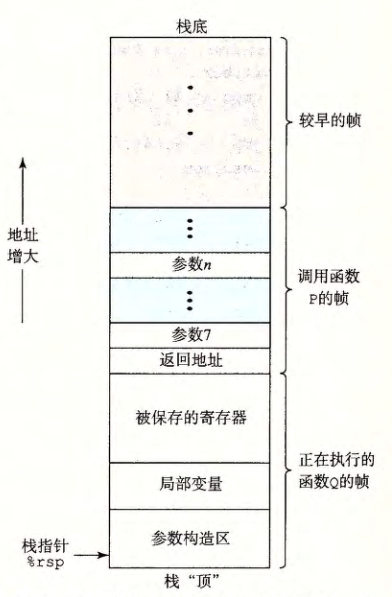
\includegraphics[width=0.4\textwidth]{stack-structure.png}
\end{figure}

\subsubsection{转移控制}

将控制从函数P转移到函数Q只需要简单地把程序计数器设置为Q的代码的起始位置。
不过,当稍后从Q返回的时候,处理器必须记录好它需要继续P的执行的代码位置。

\begin{table}[H]
    \centering
    \begin{tabular}{|c c|c|}
        \hline
        \multicolumn{2}{|c|}{\textbf{指令}} & \textbf{描述} \\
        \hline
        call & Label & 过程调用 \\
        call & *Operand & 过程调用 \\
        \hline
        ret &  & 从过程调用中返回 \\
        \hline
    \end{tabular}
\end{table}

\subsubsection{数据传送}

当调用一个过程时,除了要把控制传递给它并在过程返回时再传递回来之外,过程调用还可能包括把数据作为参数传递。
x86-64中,可以通过寄存器最多传递6个整型(例如整数和指针)参数,大部分过程间的数据传送是通过寄存器实现的。

寄存器的使用是有特殊顺序的,寄存器使用的名字取决于要传递的数据类型的大小。

\begin{table}[H]
    \centering
    \begin{tabular}{|c|c|c|c|c|c|c|}
        \hline
        \multirow{2}{*}{\textbf{操作数大小(位)}} & \multicolumn{6}{c|}{\textbf{参数数量}} \\
        \cline{2-7}
        & 1 & 2 & 3 & 4 & 5 & 6 \\
        \hline
        64 & \%rdi & \%rsi & \%rdx & \%rcx & \%r8 & \%r9 \\
        \hline
        32 & \%edi & \%esi & \%edx & \%ecx & \%r8d & \%r9d \\
        \hline
        16 & \%di & \%si & \%dx & \%cx & \%r8w & \%r9w \\
        \hline
        8 & \%dil & \%sil & \%dl & \%cl & \%r8b & \%r9b \\
        \hline
    \end{tabular}
\end{table}

如果一个函数有大于6个整型参数,超出6个的部分就要通过栈来传递。

\paragraph{栈上的局部存储}

有些时候,局部数据必须存放在内存中,常见的情况包括:
\begin{itemize}
    \item 寄存器不足够存放所有的本地数据。
    \item 对一个局部变量使用地址运算符‘&’,因此必须能够为它产生一个地址。
    \item 某些局部变量是数组或结构,因此必须能够通过数组或结构引用被访问到。
\end{itemize}

\paragraph{寄存器中的局部存储空间}

寄存器组是唯一被所有过程共享的资源,我们需要确保当一个过程(调用者)调用另一个过程(被调用者)时,被调用者不会覆盖调用者稍后会使用的寄存器值。

根据惯例,寄存器rbx、rbp和r12-r15被划分为\emph{被调用者保存寄存器}。
当过程P调用过程Q时,Q必须保存这些寄存器的值,保证它们的值在Q返回到P时与Q被调用时是一样的。
所有其他的寄存器,除了栈指针rsp,都分类为\emph{调用者保存寄存器}。

\subsection{数据结构}

\newpage
